\documentclass[a4paper]{article}

\usepackage{graphicx}
\usepackage[colorlinks=true]{hyperref}
\usepackage{paralist}
\usepackage[official]{eurosym}
\def\figline{\rule{\textwidth}{0.3mm}}

\begin{document}



\title{PACT: \\ {\large Programming ${\land}$ Algorithms $\Rightarrow$ Computational Thinking}}

\author{Aidan Mooney, Joseph Duffin, Rosemary Monahan and James F. Power}

\begin{figure}\centering

\includegraphics[height=.2\textheight]{nuim_large.jpg}
\end{figure}

\maketitle

\section{Introduction}
The PACT programme is a partnership between researchers in the Department of Computer Science at NUI Maynooth and teachers at selected post primary schools around the country.   Starting in September 2013 a number of Irish secondary schools took part in a pilot study, delivering material prepared by the PACT team to transition year students.

Initially the focus of this partnership is on teaching programming to transition year students, but ultimately the goal is to develop a framework for delivering a short course on \textit{computational thinking} as part of the new Junior Certificate cycle.


\section{Background and Motivation} \label{Background}

NUI Maynooth has been delivering programmes in Computer Science at undergraduate and postgraduate level for 25 years and, since 2012, has been delivering a unique \textit{BSc in Computational Thinking}.  This degree is a blend of Computer Science, Mathematics and Philosophy, and aims to provide a deeper education in computing than the more traditional degrees, which often have a strong vocational orientation.  The PACT initiative aims to build on the visibility of the \textit{Computational Thinking} brand to bring the ideas at the heart of this degree to second-level students.

\paragraph{What is Computational Thinking?}

The phrase \textit{Computational Thinking} was originally coined in the context of mathematics education by by Seymour Papert \cite{papert96}, but came to prominence in Computer Science following an influential article by Jeannette M. Wing \cite{wing-cacm06}.  Wing's article described computational thinking as
\begin{quotation}
``Computational thinking builds on the power and limits of computing processes, whether they are executed by a human or by a machine.  Computational thinking confronts the riddle of machine intelligence: What can humans do better than computers? and What can computers do better than humans? Most fundamentally it addresses the question: What is computable?''
\end{quotation}


This perspective has been developed by the 
\textit{Center for Computational Thinking} at Carnegie Mellon University\footnote{\url{http://www.cs.cmu.edu/~CompThink/}}
(sponsored by Microsoft Research), and echoed in other programmes, including those by 
Google\footnote{\url{http://www.google.com/edu/computational-thinking/}} and the
\textit{International Society for Technology in Education}\footnote{\url{http://www.iste.org/learn/computational-thinking}}.

Crucial elements of this perspective are that:
\begin{compactitem}
\item Computational thinking is a way that humans, not computers, think.
\item Computational thinking is a fundamental skill for
everyone, not just for computer scientists.
\end{compactitem}


\paragraph{Computational Thinking in Schools.} \label{par:CTSchools}

There have been numerous efforts over the years to introduce computational concepts into Irish secondary schools but, at an official level, these never proceeded much beyond basic elements of information technology.  The reform of the Junior Certificate cycle offers an opportunity to get this right: a course designed by Computer Scientists to display the depth and beauty of the field in a way that can challenge and engage second-level students.  An emphasis on 
\textit{Computational Thinking} allows us to explore the key concepts the underlie Computer Science, without necessarily having to achieve the full rigour of the professional scientific discipline.

We can identify three key levels of understanding in Computer Science:
\begin{itemize}
\item \textbf{Programming} is a threshold concept in Computer Science, as it introduces some of the basic challenges of the discipline.  
\item \textbf{Algorithms} involves studying solutions in computational terms: which solutions are better, in what circumstances, and why?
\item \textbf{Computability} is the study of \textit{problems} in 
computational terms: what can be computed, and why?
\end{itemize}

The goal of the PACT programme is to guide students through the key topics in programming and algorithms towards the ultimate goal of studying the process of computation itself.

The PACT group at NUIM has collaborated with teachers across 9 secondary schools to develop a flexible module which will engage Transition Year students.  The focus of the module is not on learning facts about computers but on developing creative ideas and new ways of thinking.  Continuing feedback will be used to expand the module into a full Junior Cycle short course. 

\section{Related work} \label{sect:relWork}

The NCCA has developed a specification for eight Junior Cycle short courses for use from 2014, and one of these is 
titled \textit{Programming and Coding} \cite{ncca-prog13}.  This is a useful document as it provides an example of addressing the general skills requirements of a short course.  The computing content seems to consists of basic programming skills along with some multimedia (web page) design, with a goal of developing students teamwork skills.  

There is, however, no mention of a broader Computational Thinking agenda, nor any clear indication that the module is even intended to be scientific in nature.  From a Computer Science perspective this curriculum is quite limited in scope (just as its title would suggest), and we would seek to develop a much broader understanding of the core principles of our discipline.

\paragraph{Other initiatives similar to PACT:}

There are at least two current initiatives in Ireland that are similar in some respects to PACT:

\begin{itemize}

\item The Lero group in the University of Limerick  established an education and outreach programme starting in 2007, originally to support teaching using MIT's Scratch environment in Irish post-primary schools.  They have developed a website\footnote{\url{http://www.scratch.ie/}}
with support for primary and post-primary schools, including extensive lesson plans and teaching material, and run teacher training sessions as well as an annual competition.

While the structure of the Lero initiative is similar to ours, we believe that a graphical language like Scratch is fundamentally limited in terms of teaching programming, even though it may serve as a useful introduction to some programming concepts.  Further, the materials seem to be limited to teaching programming in Scratch, and do not seem to have a broader agenda in Computer Science or Computational Thinking.

\item Bridge21\footnote{\url{http://www.bridge21.ie/}} is an education programme based in Trinity College Dublin and supported by Google.  It claims to be based on a new model of learning that can be adapted for use in secondary schools \cite{conneely13}, and they provide professional development workshops for teachers to train in ``21st Century Computer Science Teaching Skills''. 

This initiative is directly targeting the post-primary (and Junior cycle) area, but appears to be more broadly based than our initiative, recently offering support for English, Maths and History classes.  While the specific Computer Science deliverable is vague, it seem to be based at present on programming (and the Raspberry Pi), and it is not clear what their precise CS agenda is.
\end{itemize}

Even though both of these groups are established in the field, we believe that their focus in each case lacks a clear, distinctive Computer Science perspective.  Our PACT initiative can fill this gap and, we believe, offers an alternative that provides a deeper insight into the fundamentals of our discipline.



\paragraph{Recent initiatives in the UK:}  There has been a series of interesting related work in the UK culminating in a series of reports over the last two years.


The \textit{Computing in Schools}\footnote{\url{https://royalsociety.org/education/policy/computing-in-schools/}} project was an initiative coordinated by the Royal Society in cooperation with 18 UK universities  as well as several industry bodies culminating in a report published in January 2012 \cite{rcs-cis12}.  It notes the limitations of the previous National Curriculum in ICT, and emphasises the need to switch to `creative, rigorous
and challenging Computer Science'.  It identifies that Computer Science is a rigorous academic discipline and that significant investment in continuing professional
development for teachers will be needed.  

Their suggested `terminological reform'  encapsulates the understood position of Computer Science from our perspective, but is nonetheless worth replicating here since it is not widely understood outside the discipline (Figure \ref{ref:terminology}).  While much of this document is discusses long-term funding needs and is thus directed at policy-makers, the emphasis on depth and rigour is similar in spirit to our PACT initiative.

\begin{figure}\centering
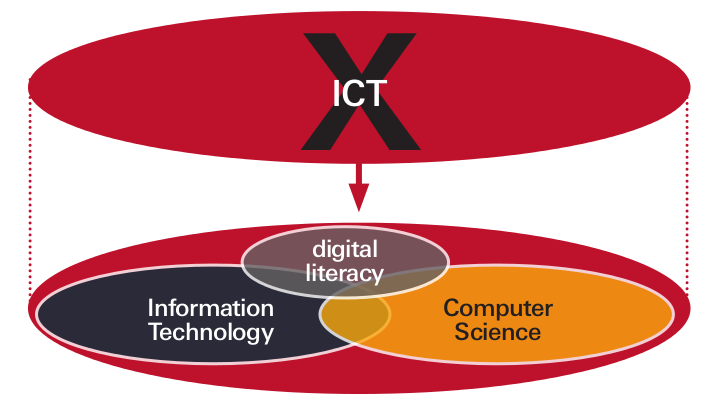
\includegraphics[width=.9\textwidth]{terminology.png}
\caption{Replacing `ICT': suggested terminological reform from the 
\textit{Computing in Schools} initiative, emphasising the distinctive identity of Computer Science.}
\label{ref:terminology}
\end{figure}

The \textit{Computing at School}\footnote{\url{http://www.computingatschool.org.uk/}} initiative by the British Computer Society has produced a curriculum for schools that has been endorsed by Microsoft, Google and Intellect an d published in March 2012 \cite{bcs-curr12}.  This curriculum develops a clear agenda for computing-related concepts, stratified in five stages that cover primary and post primary education.  It clearly identifies Computer Science as a STEM discipline, distinguishes it from Information Technology, and emphasises core skills such as programming as well as more abstract skills such as designing algorithms and computational thinking.  While this \textit{Computing at School} is a much more ambitious agenda that the PACT initiative, it shares many of the themes and goals of PACT.

The summary of key points from a related \textit{Computing at School} briefing note published in November 2011 \cite{cat-brief-11} is worth quoting in full, since it covers many of the key points that have informed the PACT initiative (see Figure \ref{fig:points}).  

\begin{figure}
\figline
\begin{compactitem}
\item It is vital to make a clear distinction between Computer Science as a rigorous subject
discipline on the one hand, and IT applications and/or digital literacy on the other.
\item Many countries, from the USA to India, routinely make Computer Science available to young people at school from an early age.
\item There is increasing clarity that ``Computer Science'' means a lot more than ``Learn to program
         in Java or C++''. Programming is central to computing, but the underlying principles of
          algorithms, data structures, and computational thinking skills are both more fundamental
         and more durable.
\item The confusion between Computer Science and ICT skills means that ICT is often delivered by
   non-specialists. Meanwhile, the continuing strong employer demand for IT professionals
  reduces the supply of well-qualified potential teachers. These factors conspire to mean that
 ICT/Computing teachers are under-valued and under-qualified. There is a desperate need
for teacher training in Computer Science.
\end{compactitem}
\figline
\caption{Key points identified by the \textit{Computing at Schools} group based on a study of the international experience with teaching computing in schools (direct quotation from \cite{cat-brief-11}).}
\label{fig:points}
\end{figure}

\paragraph{Recent initiatives in the US:}  

In the US, much of the focus on K-12 CS edutaion is directed through the ACM-supported \textit{Computer Science Teachers Association} (CSTA)\footnote{\url{http://csta.acm.org/}}.  In their 2010 report they identify gaps in state standards for CS education, as well as major terminological confusion between digital literacy, information technology and computer science \cite{csta-roe10}.  They identify the need to establish Computer Science as an academic discipline within the STEM fields; the key topics they identify in CS education are shown in Figure \ref{fig:cse}.
The CSTA has established a \textit{Computational Thinking Task Force} to collect and disseminate teaching resources and projects in this area.

\begin{figure}
\figline\\
\centerline{\begin{tabular}{p{.9\textwidth}}
\textbf{Computer science education} includes the following
elements: design (both software and hardware), creation
of digital artifacts, abstraction, logic, algorithm development and implementation, programming paradigms and
languages, theoretical foundations, networks, graphics,
databases and information retrieval, information security
and privacy, artificial intelligence, the relationship between computing and mathematics, the limits of computation, applications in information technology and information systems, and social impacts of computing.
\end{tabular}}
\figline
\caption{Elements of Computer Science education for K-12, as identified by the CSTA (direct quotation from \cite{csta-roe10}).}
\label{fig:cse}
\end{figure}


The CS10K community\footnote{\url{http://cs10kcommunity.org/}}
aims to place 10,000 qualified computer science teachers into high schools to broaden access to computing education.  They have developed resources in two streams: \emph{Exploring Computer Science} covers problem solving, web design, programming (using \textit{Scratch}) and robotics, while \emph{Computer Science Principles} has a stronger  programming and algorithms focus (and uses \textit{App Inventor}, a Scratch-like environment for Android app development).
The CS10K Project is supported by the National Science Foundation as part of its Computing Education for the 21st Century (CE21) programme.

As a further development, \textit{Computer Science: Principles}\footnote{\url{csprinciples.org}} is a
proposed AP course being developed by the College Board, descigned as an ``introductory college-level course	for	everyone'' \cite{Astrachan:2012}.  It emphasises what it calls \textit{computational thinking practices}, such as developing computational artefacts, creativity, abstraction and communication.

Each of these courses is considerably broader than that proposed by our PACT initiative, but many of the topics overlap, and it should be possible to reuse some of the rich collection of resources they have developed.
 
\bigskip
In summary, the principal initiatives from the UK, USA and other countries emphasise: 
\begin{compactitem}
\item the need to reform CS education at post-primary level,
\item the need to distinguish clearly between digital literacy, information technology and CS,
\item the need to teach CS concepts as a rigorous academic discipline within the STEM subjects.
\end{compactitem}


\section{Our work to date} \label{sect:OurWork}
During the Summer of 2013 a number of schools were approached to gauge if there was interest in running such a pilot programme. The schools which came on board were:
\begin{compactitem}
  \item Maynooth Post Primary School, Co. Kildare.
  \item Pobalscoil Neasain, Baldoyle, Dublin 13.
  \item Confey Community College, Leixlip, Co. Kildare.
  \item Castelcomer Community School, Co. Kilkenny.
  \item Scoil Mhuire Community School, Clane, Co. Kildare.
  \item Jesus and Mary College, Goatstown, Dublin 14.
  \item Salesian College, Celbridge, Co. Kildare.
\end{compactitem}

At least one teacher from each of these schools agreed to participate in the pilot programme. 

\paragraph{Teacher training sessions:}
The PACT team began to structure the content for the pilot programme and on the 25th of May and the 1st June 2013 two training sessions took place in NUIM. These sessions involved introducing the teachers to the content within the programme and also getting to know each other. It was hoped that a community of knowledge and learning would be created between all the teachers as they progressed with the pilot.

A Moodle system was hosted in the Department of Computer Science to store the content that was delivered in the training sessions. The content was divided in to five components, namely:

\begin{compactenum}
  \item Introduction to Python I.
  \item Introduction to Python II.
  \item Algorithms.
  \item Graphics.
  \item Recursion and self-reference.
\end{compactenum}


The content was based on the \textit{Python} programming language\footnote{\url{https://www.python.org/}}. 
\textit{Python} is a dynamically-typed programming language that is popular in the CoderDojos as a first programming language, but also is used in a number of professional and scientific applications.  The choice of programming language is not essential for the syllabus, and we envisage providing options for teachers who wish to develop using other languages such as \textit{Processing} or \textit{Haskell}.

Components 1 and 2 of the training sessions covered the basics of installation of \textit{Python} and also looked at how to create and run programs written in \textit{Python}. They looked at the main features of the language and gave sample programs for the teachers to use. 
An exercise book was created for all lessons within these sections which the teacher could use in class to get their students working in \textit{Python}. In total 19 PowerPoint presentations were prepared for these sections which the teacher could break up into whatever format they felt worked for them. 

Component 3 focused on algorithms and the process of analysing problems to devise abstract computational solutions.  It showed how to write a step by step procedure to solve some classic problems in Computer Science. Component 4 looked at generating simple 2-D graphics using the \textit{Pygame} set of modules. This section focused on allowing the participants to create fully featured games in the \textit{Python} language, and can provide a useful focus for project-based programming work.  Component 5 covered topics related to recursion which has been defined as ``the process of repeating items in a self-similar way" and is fundamental to the core theory of Computer Science. \\

%\newline


%\paragraph{Competition:}
%Towards the end of the academic year 2013-14 we are going to host a competition which is open to all the students who were involved with the PACT pilot programme. This competition is aimed at providing examples of best practice and each school participating in the pilot is invited to select up to two teams, consisting of 3-5 students, to participate in the competition. The selection of teams and team members is entirely at the discretion of the schools. Participants in the competition should highlight explicitly how their experience with the PACT programme has contributed to two or more of the six key areas identified by the NCCA \cite{ncca2013}, namely:

%\begin{compactenum}
%  \item Managing Myself.
%  \item Staying Well.
%  \item Communicating.
%  \item Being Creative.
%  \item Working with Others.
%  \item Managing Information and Thinking.
%\end{compactenum}

\section{Feedback} \label{label:Feedback}
Towards the end of the 2013-14 academic year the PACT team organised for surveys to be made available for teachers who taught the PACT material \footnote{\url{https://docs.google.com/forms/d/1-17vL9ZxeTVIKfJcsNm0rMDiJsISttpcA2Cm5VQVLvk/viewform}} and also for the students who took the module \footnote{\url{https://docs.google.com/forms/d/1_l0fmD1C9aLeD7pwdl5a9Im4Or3ZzuvHe6MfsD5KOs0/viewform}}. 

To date there have been $62$ student responses and $7$ teacher responses.  These $7$ teachers represented $5$ schools within these $5$ schools $294$ took the module across $13$ class groups. There was one all-girls school, one all-boys school and three mixed schools. It is clear from the teacher responses that unless there is complete support and buy-in from the management of the school courses like this will not survive.  One teacher commented that ``The pupils were very keen to learn how programming was being used in the working world", something that the PACT team has tried to incorporate in to the module.

\textbf{These figures will need to be updated when all submissions are received.}

No streaming took place in any of the class groups which took this module. However, one teacher noted that there was ``No streaming, but the students choose to take the course. 2/3 of them were ordinary level maths students and they could not get their head around the logical thinking required to program and they ended up moving over to Scratch instead". All of the classes covered Python 1 and Python 2 with most also covering Algorithms with some covering Self-Reference and Graphics.

Initial analysis of the feedback suggests that almost $65\%$ of the students found that ``taking part in this pilot programme has been beneficial to you"? $80\%$ of the students who replied to the survey said that this module was very different compared to other subjects they have taken in school.

Asked as to what the students enjoyed in the module some of the positive responses were:

\begin{compactitem}
  \item ``It was different to other things on the computer". 
  \item ``I enjoyed being able to tell the computer to do something and it would do it".
  \item ``Learning the basics of coding".
  \item ``I most enjoyed writing codes that had a visual result like the turtle code".
\end{compactitem}  

When the students were asked to provide some overall feedback on the programme and any suggestions on how this could be improved, some of the responses were:

\begin{compactitem}
  \item ``I feel it should be continued as it seemed very beneficial and helpful for the other lads but it just wasn't for me really . One way I think it could be improved would be if there was some kind of game involved rather than just doing exercises all the time.". 
  \item ``It was very enjoyable and different. Sometimes it was very hard but extremely good and beneficial".
  \item ``It was good to learn how to programme/ make programmes.".
  \item ``I thought the whole program was good, and I did look forward to each class. I think that the questions that are posed to do should be a bit more practical and try give the user more of feeling of what the computer is actually doing. Example of where I previously learned code can be seen in Lua, from ComputerCraft. There is a ComputerCraft Edu that teaches people lua. This could be used to show people how code works and impacts better that through the IDLE.".
\end{compactitem}  


\section{Future Work} \label{Sect:FutWork}
As of the 15th May 2014 we have already received interest from the following schools:
\begin{compactitem}
  \item Tallaght Community School, Dublin. 
  \item Sandford Park, Ranelagh, Dublin.
  \item St. Munchin's College, Limerick.
  \item Beneavin College, Finglas, Dublin.
  \item Coláiste Cois Life, Lucan, Dublin.
  \item St. Wolstans Community School, Celbridge, Kildare. 
  \item Colaiste Chiarain, Leixlip, Kildare. 
  \item St. Mel's College, Longford.
\end{compactitem}  

The majority of these schools have approached us directly from seeing our webpage or from teachers who are involved in the pilot programme this year. We have also distributed letters to 10 schools based on their proximity to NUIM that are not currently enrolled in PACT. We hope to run this programme again for the academic year 2014-15 with a larger number of schools and take on board the feedback received from the teachers and students in the first year.

During the Summer of 2014 a student intern will be working with the PACT team to develop further resources for teachers, develop a wiki with resources for students and analyse possible future developments for PACT, amongst other things.


\section{Future funding initiative} \label{Sect:FutFunding}
The Erasmus+ Programme which commenced on the 1st January 2014 offers the opportunity for Strategic Partnerships for organisations involved in school education. As outlined in Section \ref{par:CTSchools}, other Irish and international initiatives in teaching basic programming skills and multimedia design, aim to develop student teamwork and communication skills. While these initiatives are welcome, they are limited in that they do not address the broader principles of Computer Science. Initiatives to introduce Computer Science to schools in Europe and in the USA have concluded that there is a need to reform Computer Science education at post-primary level to promote  both Computer Science and digital literacy. 

The NUIM PACT programme provides the ground work for such a reform in Computer Science. It places NUIM in the ideal position of leading an Erasmus+ Strategic Partnership (under Key Activity 2) which would be funded for 3 years. These partnerships focus on activities designed to improve education provision across the participating countries, promoting cross-sectoral cooperation and addressing policy objectives, challenges and the needs of a specific field such as post-primary and third-level education.  Through such a strategic partnership with schools, universities and industry, we will be empowered to implement joint initiatives on programme curriculum and teaching training, as well as promoting exchange of experience and know-how. In 2014 the allocation of funding in Ireland for such a partnership was \euro 450,000. It is expected that the funding available n 2015 will be increased and the application deadline will be in April 2015.  



\section{Contact Us} \label{Sect:ContactUs}
The PACT team can be contacted at the following email address: \url{pact@cs.nuim.ie}.

The member of the Computer Science department currently involved in the PACT initiative are:
Aidan Mooney (coordinator),
Susan Bergin,
Joe Duffin,
Phil Maguire,
Rosemary Monahan,
Tom Naughton and
James F. Power. 




Our website is: \url{http://www.cs.nuim.ie/pact}.

\bibliographystyle{unsrt}%{plain}
\bibliography{ref}
\end{document}
